\documentclass[tikz,border=3.14mm]{standalone}
\usepackage{tikz}

\begin{document}
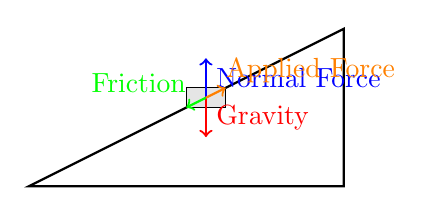
\begin{tikzpicture}

% Drawing the inclined plane
\draw[thick] (0,0) -- (4,0) -- (4,2) -- cycle;
% Drawing the block
\draw[fill=gray!20] (2,1) rectangle (2.5,1.25);
% Forces on the block
\draw[->,red,thick] (2.25,1.125) -- (2.25,0.625) node [midway,right] {Gravity}; % Gravity
\draw[->,blue,thick] (2.25,1.125) -- (2.25,1.625) node [midway,right] {Normal Force}; % Normal force
\draw[->,green,thick] (2.25,1.125) -- (2,1) node [midway,above left] {Friction}; % Friction
\draw[->,orange,thick] (2.25,1.125) -- (2.5,1.25) node [midway,above right] {Applied Force}; % Applied force

\end{tikzpicture}
\end{document}